% TEXINPUTS=templates/LaTeX2e//: pdflatex paper1_iberamia_timeformer.tex
% TEXINPUTS=templates/LaTeX2e//: bibtex paper1_iberamia_timeformer
% TEXINPUTS=templates/LaTeX2e//: pdflatex paper1_iberamia_timeformer.tex
% TEXINPUTS=templates/LaTeX2e//: pdflatex paper1_iberamia_timeformer.tex
%
% This file is intentionally a planning skeleton, not a full manuscript draft.
\documentclass[runningheads]{llncs}

\usepackage[T1]{fontenc}
\usepackage{graphicx}
\usepackage{amsmath}
\usepackage{amssymb}
\usepackage{booktabs}

\begin{document}

\title{Time-blind by Design: Diagnosing Temporal Traceability in Transformer Representations}
\titlerunning{Time-blind by Design: Temporal Traceability in Transformer Representations}

\author{Jefferson de Oliveira Silva\inst{1,2}}
\authorrunning{J. O. Silva}

\institute{Instituto de Tecnologia e Liderança, São Paulo, Brazil\\
\email{jefferson.oliveira@prof.inteli.edu.br} \and
Pontifícia Universidade Católica de São Paulo, São Paulo, Brazil}

\maketitle

\begin{abstract}
Words do not preserve fixed meanings across time. Without suitable
representations, we cannot directly compare uses of \emph{gay} in 1920 and
1980. Yet time-conditioned transformers have rarely been
tested on whether the neighborhoods of their contextual representations reflect
how a word is used in the requested period. Recovering the period identifier
alone does not ensure this property, which we call \emph{temporal
traceability}. We introduce a controlled test suite with predefined stable,
drifting, and bifurcating usage trajectories to evaluate it.

Three findings emerge. Giving the model period information more than doubles
the change in neighborhood composition for drifting subjects relative to the
non-temporal baseline. However, direct addition of the period vector and a
learned token--period projection produce equivalent average changes when nearby
verbs and objects are reliable cues; a difference appears when those cues are
degraded. Finally, memory ablations show that label-derived history improves
later-period classification accuracy, whereas mean pooling and two
\(k\)-means centers do not surpass Token-Time.

\keywords{Temporal semantics \and Semantic change \and Transformer models \and Traceability \and Diagnostic evaluation}
\end{abstract}

\section{Introduction}

Word meanings change over time. In 1900, \emph{broadcast}
referred to scattering seeds across a field; today it describes a social media
post reaching millions. Lexical semantic change detection (LSCD) usually learns
a separate representation space for each period and aligns these spaces before
comparing a word across time~\cite{schlechtweg2020semeval,tahmasebi2021survey}.
These methods have produced important benchmarks and results, but usually
summarize a target's change as a similarity score. Thus,
the 1900 and 2020 representations of \emph{broadcast} come from separate,
aligned spaces rather than from period-specific queries to one model.

We call contextual representations \emph{temporally traceable} when they satisfy
two conditions: representations of the same word at different periods are
directly comparable, and their nearest neighbors change as the word's use
changes.
Consider \emph{gay}, which in the early twentieth century was mainly associated
with \emph{cheerful} and \emph{merry}, and by the late twentieth century with
\emph{queer} and \emph{lesbian}~\cite{hamilton2016diachronic}. A traceable model
should therefore place uses of \emph{gay} from 1920 closer to contexts associated
with \emph{cheerful} and \emph{merry}, and uses from 1980 closer to contexts
associated with \emph{queer} and \emph{lesbian}. Such comparisons can support
socially relevant analyses, including whether a word moved toward or away from
stigmatized terms.

In our controlled corpus, we specify in advance how often each subject appears
with each of two context groups across ten periods. These schedules define
stable, drifting, and bifurcating usage trajectories. This control lets us test
whether a representational change comes from the architecture rather than from
uncontrolled differences in word frequency, genre, or corpus composition. Four
diagnostics test whether representations recover the context group that
generated a sentence, whether their neighborhoods follow the predefined
trajectory, whether changing only the period changes a prediction, and whether
they transfer to later periods.

With this suite we evaluate one non-temporal baseline (Standard) and three
time-aware architectures. Additive adds the same period vector at every
position. Token-Time instead learns a projection that combines each token with
the period before the encoder. Memory-Augmented also lets the subject input
consult summaries from earlier periods. We test whether these designs improve
temporal traceability and which design choices matter.

The paper makes four contributions. (1) We define temporal traceability through
changes in the neighborhoods of comparable, period-conditioned contextual
representations. (2) We introduce a controlled corpus with three usage
trajectories and four diagnostics that separate neighborhood composition from
label prediction. (3) We show that all time-aware architectures more than
double the neighborhood shift for drifting subjects; Additive and Token-Time
are equivalent with reliable cues, while Token-Time has a small classifier
advantage when they are fully uninformative. (4) Memory ablations show that an
oracle memory built from generating-group labels improves later-period
classification, whereas representation-derived means and two \(k\)-means
centers do not surpass Token-Time.

\section{Related Work}
% Target length: under 1 page.
Most computational studies of meaning change use lexical semantic change
detection (LSCD). Diachronic word embeddings~\cite{hamilton2016diachronic}
learn one vector space per time slice, align the separately trained spaces, and
track changes in a word's neighbors. Our approach instead obtains
period-conditioned contextual representations from one model rather than
comparing period-specific spaces.
Standard benchmarks evaluate LSCD~\cite{schlechtweg2020semeval,tahmasebi2021survey}.
Natural-corpus scores may reflect shifts in frequency or genre, and benchmark
construction requires manual annotation even for modern
corpora~\cite{zamora2022lscdiscovery}. In our controlled corpus, we set
trajectories in advance, so corpus composition is fixed across architectures.

Temporal neural language models instead condition one model on time. Prior work
uses timestamps for knowledge-intensive QA, masked language
modeling, or period-stratified downstream
evaluation~\cite{dhingra2022timeaware,rosin2022timemasking,loureiro2022timelms}.
These studies show that time conditioning can improve period-appropriate
predictions, but do not test whether the same word's neighborhoods match each
period within one model.

Finally, words can develop new senses that coexist with older
ones~\cite{giulianelli2020analysing}. Averaging representations of two senses may
produce a vector that represents neither one. Our bifurcating trajectories test
whether a mean summary preserves this structure; the memory ablations compare
alternatives.

\section{Controlled Diagnostic Suite}
% Target length: 1.0 page.
We construct a corpus of subject--verb--object (SVO) sentences spanning ten
periods. Every sentence consists of one subject, one verb, and one object. We
divide the 8 verbs and 8 objects
into two groups, $N_1$ and $N_2$, which provide distinct contextual cues:
we assign \(\{V1,\ldots,V4\}\) and \(\{O1,\ldots,O4\}\) as the canonical
vocabulary of $N_1$, and \(\{V5,\ldots,V8\}\) and \(\{O5,\ldots,O8\}\) as that
of $N_2$. Without cue noise, an $N_1$ sentence looks like
\texttt{S5 V2 O3}, while an $N_2$ sentence looks like \texttt{S5 V6 O8}; the
subject token is the same in both cases, but its co-occurring words differ. For
each subject $s$ and period $t$, \(P(N_1 \mid s,t)\) is the probability of
selecting $N_1$ as the generating group. The ten probabilities from \(t0\) to
\(t9\) define the subject's trajectory.

\begin{figure}[!h]
\centering
\includegraphics[width=\textwidth]{outputs/figures/figure1_benchmark_design.pdf}
\caption{Controlled diagnostic suite overview. \emph{Left}: SVO sentences for a drifting
subject across three periods; an $N_1$ verb appearing in a sentence generated from $N_2$
at \(t7\) (marked \({\ast}\)) illustrates the deliberate noise in contextual cues.
\emph{Center}: predefined \(P(N_1 \mid s, t)\) trajectories for Stable (flat),
Drift (monotonic), and Bifurcating (levelling at 0.5) subjects across
\(t0\)--\(t9\). \emph{Right}: nearest-neighbor behavior expected from the
predefined trajectory.}
\label{fig:benchmark-design}
\end{figure}

Figure~\ref{fig:benchmark-design} (center) shows the three predefined trajectory
classes. Stable subjects maintain an approximately constant \(P(N_1 \mid s, t)\)
throughout. Drift subjects follow a monotonic trajectory from near-exclusive
$N_1$ (\(P(N_1 \mid s, t) \approx 1\) at \(t0\)) to near-exclusive $N_2$
(\(P(N_1 \mid s, t) \approx 0\) at \(t9\)). A drifting subject is therefore more
likely to appear in sentences such as \texttt{S5 V2 O3} early on and
\texttt{S5 V6 O8} near the final period. Bifurcating subjects begin in $N_1$
and move toward a mixed state (\(P(N_1 \mid s, t) \approx 0.5\)) where sentences
are generated from both groups with equal probability, approximating two coexisting senses. The
suite contains 10 subjects per class.

To generate a sentence for subject $s$ at period $t$, we first sample $N_1$ or
$N_2$ according to \(P(N_1\mid s,t)\). We store the sampled group as
\texttt{true\_context}. We then draw the verb and object independently: each
comes from the sampled group with 75\% probability and from the opposite group
with 25\% probability (Figure~\ref{fig:benchmark-design}, left). The accompanying
words are therefore informative but imperfect cues. \texttt{true\_context} is
not used in MLM training and is available only to the diagnostics.

All architectures use the same corpus and known trajectories, so differences
between them cannot result from frequency, genre, or corpus composition. Because
\(P(N_1 \mid s,t)\) is known, we can test whether representation neighborhoods
follow the process that generated the corpus. The Discussion explains how these
diagnostics would need to change for natural corpora.

The experiments use four evaluation settings. The standard cue setting uses the
75\% cue reliability described above and matches masked language modeling (MLM)
training. The ambiguous cue setting reduces this probability to 50\%, so verbs
and objects do not identify the generating group on average. The contrastive set
presents the same masked-verb subject--object frame with two period identifiers
and tests whether changing only the period changes the preferred group. The
later-period transfer set contains \(t8\)--\(t9\), which are excluded from MLM
training on \(t0\)--\(t7\).

\section{Time-Aware Architectures}
% Target length: 2.0 pages.
We evaluate one non-temporal baseline and three time-aware architectures,
all using the same Transformer encoder configuration. Standard (no period input) is
the non-temporal baseline. The three time-aware architectures differ in how
they introduce time: Additive gives every token the same period vector;
Token-Time uses a learned joint token--period projection before the encoder; and
Memory-Augmented also lets the subject consult summaries of earlier periods.

All models follow the same pipeline based on the Transformer
encoder~\cite{vaswani2017attention}. A sentence is tokenized as
\texttt{[CLS] S V O [SEP]}. The learned token embedding \(e(w_i)\) is combined
with position and, when available, period information to form the encoder input
\(z_i \in \mathbb{R}^d\). The sequence \((z_1,\ldots,z_n)\) is processed by a
Transformer encoder, and the final hidden state at the subject position,
\[
  (h_1,\ldots,h_n) = \mathrm{Encoder}(z_1,\ldots,z_n),
  \qquad h_s = h_{\mathrm{subj}},
\]
is the contextual representation of that subject occurrence inspected by the diagnostics. All
models are trained with MLM~\cite{devlin2019bert}: some tokens are masked, and the model reconstructs
them from the remaining tokens and, when available, the period input. The
variants differ in how they inject temporal information before the encoder.

The three time-aware models use the same type of period encoding. Within each
model, \(\tau(t) \in \mathbb{R}^d\) is a learned projection of sinusoidal
features of \(t/(T-1)\), where \(T=10\) is the number of corpus periods. It is
distinct from the learned position embedding \(p_i\), which marks each token's
position.
Additive and Token-Time differ in how they combine \(\tau(t)\) with token
identity; Memory-Augmented lets the subject input consult summaries from
earlier periods. Figure~\ref{fig:architecture} summarizes the comparison.

\begin{figure}[t]
\centering
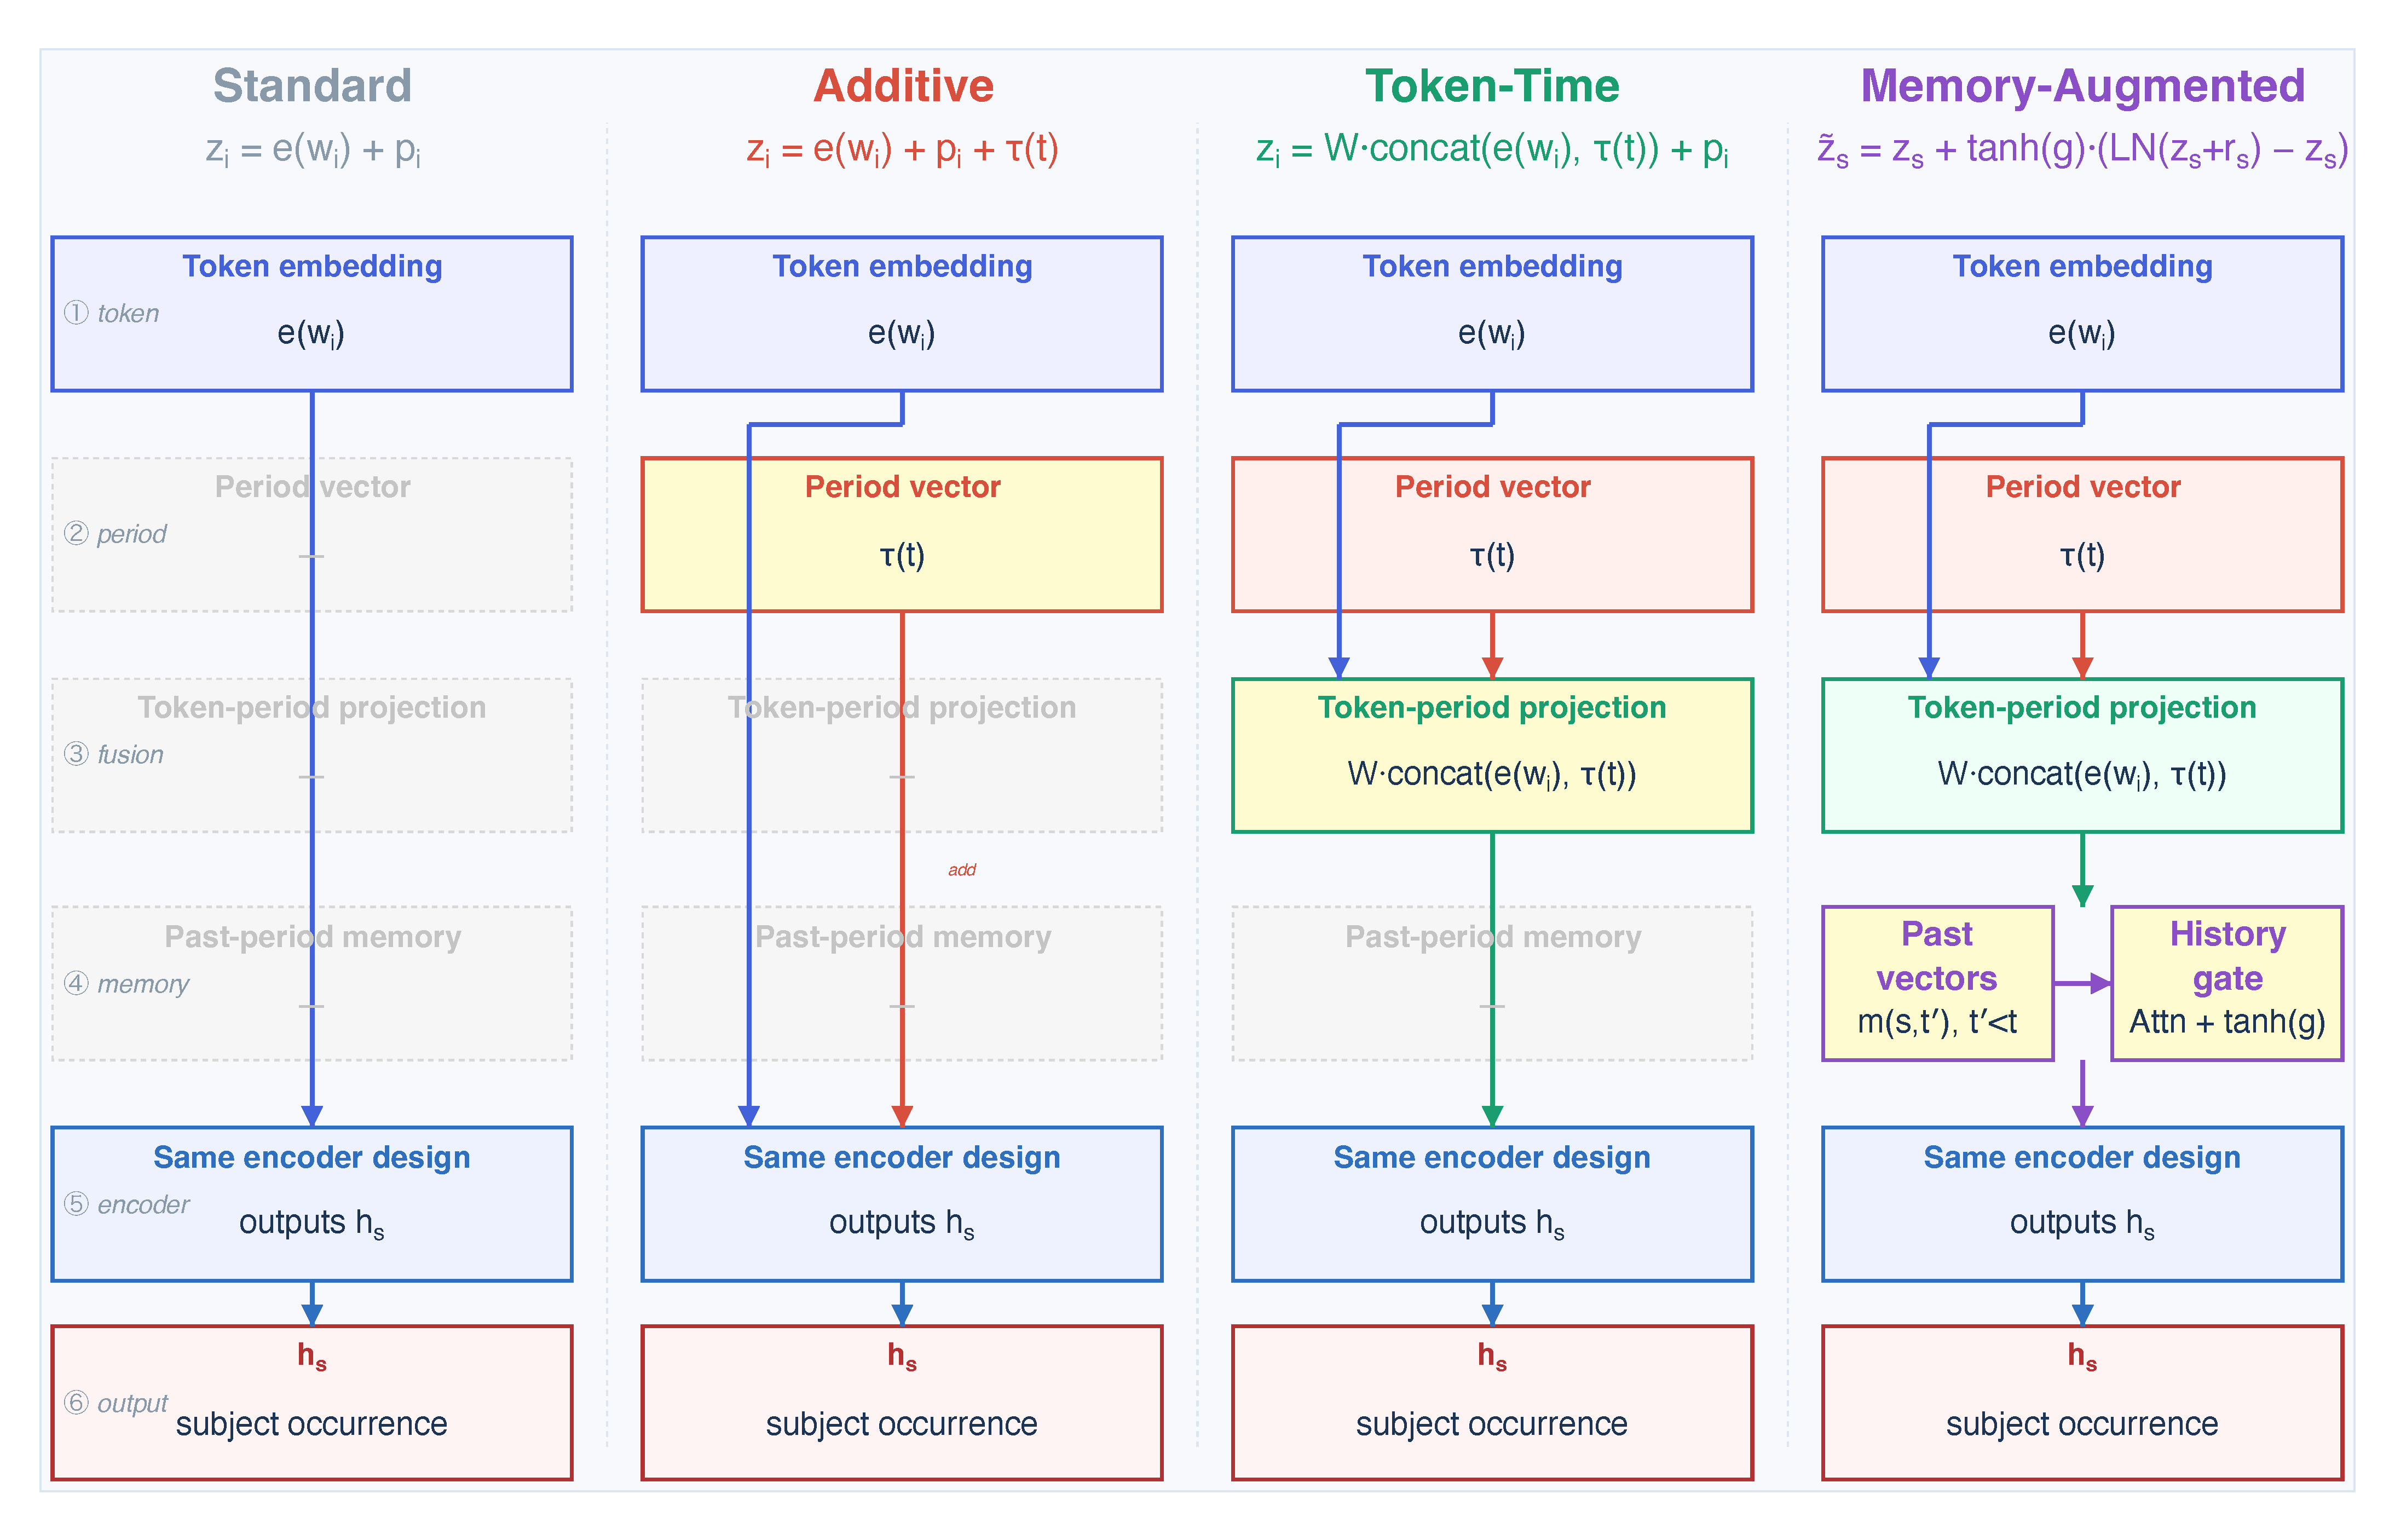
\includegraphics[width=\textwidth]{outputs/figures/figure2_architecture_detail.pdf}
\caption{Architecture comparison. \textbf{Standard}: no temporal signal.
\textbf{Additive}: adds the period vector to every token. \textbf{Token-Time}:
uses a joint token--period projection. \textbf{Memory-Augmented}: adds
past-period summaries and attention over them. New components are yellow;
dashed grey boxes are inactive.}
\label{fig:architecture}
\end{figure}

\subsection{Baseline: Standard Transformer}
Standard is the control architecture: no period signal is available, so any temporal
behavior must arise from changes in the observed words alone.
\[
  z_i = e(w_i) + p_i .
\]

\subsection{Additive Time-Conditioned Transformer}
Additive tests the simplest use of time: adding the same period vector
\(\tau(t)\) to every token:

\[
  z_i = e(w_i) + p_i + \tau(t).
\]

\texttt{S5 V2 O3} therefore receives different inputs at \(t0\) and \(t9\):
each token is combined with \(\tau(0)\) or \(\tau(9)\). The same period vector
is added at every position, so time enters each token in the same way.

\subsection{Token-Time Transformer}
Token-Time tests a learned alternative to direct addition. It concatenates each
token embedding with \(\tau(t)\) and projects the resulting \(2d\)-dimensional
vector back to \(d\) dimensions:

\[
  z_i = W \cdot \operatorname{concat}\!\left(e(w_i), \tau(t)\right) + p_i ,
\]

where \(\operatorname{concat}\) joins the two \(d\)-dimensional vectors into a
\(2d\)-dimensional vector, and the learned projection matrix
\(W \in \mathbb{R}^{d \times 2d}\) maps it back to \(d\) dimensions. The
comparison with Additive tests whether this projection helps beyond adding the
period vector directly.

\subsection{Memory-Augmented Extension}
The Memory-Augmented extension tests whether representations from earlier
periods add useful information beyond the current token--period input. It
begins with the same encoder inputs as Token-Time. For a sentence containing
\texttt{S5} at \(t7\), it builds encoder inputs for
\texttt{[CLS] S5 V O [SEP]} and modifies only the subject input before the
Transformer encoder sees the sentence.

The memory stores one past-period mean summary
\(m(s,t)\) for each subject and period. This vector is the mean of the final
hidden states \(h_s\) from MLM training sentences containing subject \(s\) at
period \(t\). When processing a sentence at period \(t\), the model can access
only summary vectors from earlier periods. At \(t7\), for example, it can use
the \texttt{S5} vectors from \(t0\) through \(t6\), but not from \(t7\) or
later.

The model uses attention to combine these past vectors. The current subject
input \(z_s\) is the attention query, while \(M_s\), with one past-period vector
per row, provides the keys and values:

\[
  r_s = \mathrm{Attn}(z_s, M_s, M_s).
\]

The resulting vector \(r_s\) is a weighted combination of the past-period
vectors. A learned scalar gate \(g\), bounded by \(\tanh\), controls how much
this summary changes the current subject input:

\[
  \tilde{z}_s =
  z_s + \tanh(g) \cdot
  \left(\mathrm{LN}(z_s + r_s) - z_s\right).
\]

Here, \(\mathrm{LN}\) denotes layer normalization. Because \(g\) is initialized
at zero, the extension initially behaves exactly like Token-Time. Finally,
\(\tilde{z}_s\) replaces \(z_s\) in the input sequence. Verb and object
inputs are unchanged, so the subject is the only token that enters the
encoder with information from earlier periods.

\section{Evaluation Protocol and Diagnostics}
% Target length: 1.25--1.5 pages.
We evaluate \(h_s\) with four diagnostics. Every time-aware architecture is
compared with Standard. We also compare Token-Time with Additive and
Memory-Augmented with Token-Time. These contrasts measure the effects of
providing time, using a learned projection instead of direct addition, and
consulting earlier representations.

\textbf{D1: Linear classifier~\cite{conneau2018probing}.} D1 tests whether a linear
classifier can tell from \(h_s\) whether the sentence was generated from
\(N_1\) or \(N_2\). We freeze the encoder and train the classifier on representations
from the standard cue condition. Its accuracy on these same representations is
training accuracy; the ambiguous cue condition tests it without retraining. High
accuracy does not show how the representation's nearest neighbors change across
periods.

\textbf{D2: Neighborhood composition.} For each evaluation sentence, we use
\(h_s\), the final representation of its subject, as the nearest-neighbor query. For example, for
\texttt{S12 V2 O7} at \(t0\), the query is the vector at the \texttt{S12}
position. We compare it with the representations of subject occurrences in all other
evaluation sentences and retrieve the \(k=10\) nearest by cosine similarity.
For each query, the score is the proportion of neighbors generated from $N_1$:
if 8 of the 10 neighbors come from $N_1$, the score is 0.8. We then average it
by trajectory class and period. The reported \(\Delta\) is the score at
\(t9\) minus the score at \(t0\); for example, a decrease from 0.8 to 0.2 gives
\(\Delta=-0.6\), indicating that the neighborhood composition changed from
mostly $N_1$ to mostly $N_2$. We also compare
the per-period scores with the predefined \(P(N_1 \mid s,t)\) trajectories.

\textbf{D3: Contrastive diagnostic.} D3 asks whether changing only the period changes
the masked-verb prediction in the correct direction. Each of the 29 pairs
contains the same subject--object frame at an early and a late period. For
example, the model receives \texttt{S12 [MASK] O2} at both \(t0\) and \(t9\).
At each period, we sum the predicted probabilities for the $N_1$ verbs
(\(V1\)--\(V4\)) and for the $N_2$ verbs (\(V5\)--\(V8\)). The pair counts as
a correct sign flip if the $N_1$ total is higher at \(t0\) and the $N_2$ total
is higher at \(t9\). A sign-flip rate of 0.3 means that 30\% of the pairs meet
both criteria.

\textbf{D4: Later-period transfer.} D4 trains a separate linear classifier on
standard cue representations from \(t0\)--\(t7\) and evaluates it without
retraining on separate sentences from \(t8\)--\(t9\). For example, for
\texttt{S12 V6 O7} at \(t8\), the classifier receives the vector at the
\texttt{S12} position and should identify $N_2$ as the group that generated the
sentence. Accuracy is the proportion of correct $N_1$/$N_2$ predictions.

\textbf{Auxiliary layer-wise comparison.} We also compute linear centered
kernel alignment (CKA) between the representations produced by pairs of models
on the same standard cue sentences, at the encoder input and after each encoder
layer. Higher CKA values indicate more similar representation
patterns~\cite{kornblith2019similarity}.

\textbf{Memory ablation.} For Memory-Augmented, we also test an oracle version
that replaces each representation-derived mean summary with one built from the
known generating-group labels. For example, if
80\% of a subject's training sentences at a given period come from $N_1$, its
oracle summary is \(0.8v_1+0.2v_2\), where the fixed orthogonal vectors
\(v_1\) and \(v_2\) represent $N_1$ and $N_2$. The attention and gate are
unchanged. Because the ordinary model does not receive these labels, the oracle
serves only as an analysis tool.

\paragraph{Implementation details.}
All models use the same Transformer encoder configuration: \(d=64\), 4
attention heads, 2 layers, feed-forward width 128, dropout 0.1. The period
encoding projects 32 sinusoidal features of \(t/(T-1)\) to \(d\) via a
two-layer MLP. Training uses
AdamW (lr \(=10^{-3}\), weight decay \(=10^{-2}\)) with a cosine annealing
schedule, 30 epochs, batch size 64. The corpus contains 5{,}000 SVO sentences;
MLM training uses 3{,}159 sentences from periods \(t0\)--\(t7\); 763 sentences
form the standard cue set held out from MLM training and used for D1--D2.
The D1 classifier is fitted and evaluated on this set. Its 615 sentences from
\(t0\)--\(t7\) also train the separate D4 classifier. Another 794 sentences
from \(t8\)--\(t9\) are reserved for D4 and excluded from both MLM and
classifier training. Separate validation sentences from all ten periods are used to
select the version of each model evaluated in the diagnostics. Thus, D4 tests
whether a classifier trained on \(t0\)--\(t7\) transfers to later-period sentences; it
is not a fully held-out forecast because model selection uses validation data
from \(t8\)--\(t9\).

\section{Results}
% Target length: 2.5--3.0 pages.
We report means and 95\% confidence intervals over 31 training seeds. Period
input creates the clearest separation across diagnostics; differences among the
time-aware designs are smaller and depend on the evaluation setting. For
drifting subjects, all three time-aware models change the proportion of
\(N_1\) neighbors by \(\Delta\approx-0.56\), more than twice Standard's
\(-0.221\).

\subsection{Changes in Neighborhood Composition}
% Main claim: temporal conditioning produces stronger neighborhood transitions than Standard.
% Use class-specific curves to avoid claiming stable subjects are perfectly flat.
Figure~\ref{fig:context-drift} and Table~\ref{tab:context-drift} show how the
proportion of \(N_1\) neighbors changes across periods. For drifting subjects,
Standard's mean proportion decreases by \(0.221\), with a 95\% CI of
\([-0.240,-0.203]\). Token-Time decreases by \(0.563\), more than twice as
much. Additive produces a similar decrease of \(0.567\).

Stable subjects also show more \(N_2\) neighbors, with \(\Delta\) between
\(-0.150\) and \(-0.180\). This residual change is about one-third of that for
drifting subjects (\(\Delta\approx-0.56\)): the diagnostic distinguishes the
trajectory classes, although stable subjects are not unchanged. Bifurcating
subjects fall between these cases: the time-aware models reach values near
\(0.53\) at \(t9\), close to their predefined 50--50 mixture.

We used a paired equivalence test to determine whether the Additive and
Token-Time changes in neighborhood composition are sufficiently close, rather
than merely failing to find a difference. We treated absolute differences below
\(0.05\) as equivalent. The
mean paired difference (Additive minus Token-Time) is \(-0.003\), with a 90\%
CI of \([-0.026,+0.019]\); the TOST supports equivalence
(\(p_\mathrm{TOST}<0.001\)). Equivalence also holds with the narrower margin
of \(0.034\) (\(p_\mathrm{TOST}=0.014\)).

\begin{figure}[t]
\centering
\includegraphics[width=\textwidth]{outputs/figures/figure3_context_drift.pdf}
\caption{Proportion of $N_1$ neighbors. Time-aware models produce stronger
$N_1$-to-$N_2$ changes for drifting subjects than Standard and similar
trajectories to one another. Stable subjects change less; bifurcating subjects
end between $N_1$ and $N_2$.}
\label{fig:context-drift}
\end{figure}

\begin{table}[!t]
\caption{$N_1$-neighbor proportions at \(t0\) and \(t9\) (31-seed means;
\(\Delta=t9-t0\); 95\% CI half-widths in brackets).}
\label{tab:context-drift}
\centering
\scriptsize
\renewcommand{\arraystretch}{0.88}
\setlength{\tabcolsep}{4pt}
\begin{tabular}{llccc}
\toprule
\textbf{Class} & \textbf{Model} & \textbf{t0} & \textbf{t9} & \(\boldsymbol{\Delta}\) [CI\(_{\pm}\)] \\
\midrule
Stable & Standard & 0.741 & 0.781 & $+$0.040 [$\pm$0.017] \\
       & Additive & 0.827 & 0.678 & $-$0.150 [$\pm$0.027] \\
       & Token-Time    & 0.835 & 0.655 & $-$0.180 [$\pm$0.024] \\
       & Mem-Aug. & 0.830 & 0.672 & $-$0.158 [$\pm$0.021] \\
\midrule
Drift  & Standard & 0.632 & 0.410 & $-$0.221 [$\pm$0.018] \\
       & Additive & 0.839 & 0.272 & $-$0.567 [$\pm$0.019] \\
       & Token-Time    & 0.833 & 0.269 & $-$0.563 [$\pm$0.020] \\
       & Mem-Aug. & 0.833 & 0.274 & $-$0.559 [$\pm$0.022] \\
\midrule
Bifurc. & Standard & 0.793 & 0.660 & $-$0.133 [$\pm$0.018] \\
        & Additive & 0.895 & 0.530 & $-$0.365 [$\pm$0.017] \\
        & Token-Time    & 0.891 & 0.525 & $-$0.366 [$\pm$0.016] \\
        & Mem-Aug. & 0.878 & 0.530 & $-$0.348 [$\pm$0.015] \\
\bottomrule
\end{tabular}
\end{table}

\begin{table}[t]
\caption{Main results (31-seed means; 95\% CIs in brackets). Nbr.\ \(\Delta\):
\(t9-t0\) proportion of $N_1$ neighbors for drift; Flip: D3 sign-flip rate;
Ambig./Later: classifier accuracy on \(h_s\).}
\label{tab:main-results}
\centering
\scriptsize
\renewcommand{\arraystretch}{0.88}
\setlength{\tabcolsep}{4pt}
\begin{tabular}{lcccc}
\toprule
\textbf{Model} & \textbf{Nbr.\ \(\boldsymbol{\Delta}\)} & \textbf{Flip} & \textbf{Ambig.} & \textbf{Later} \\
\midrule
Standard & $-$0.221 [$\pm$0.018] & 0.000 & 0.565 [$\pm$0.004] & 0.717 [$\pm$0.004] \\
Additive & $-$0.567 [$\pm$0.019] & 0.602 [$\pm$0.053] & 0.579 [$\pm$0.005] & 0.746 [$\pm$0.007] \\
Token-Time    & $-$0.563 [$\pm$0.020] & 0.624 [$\pm$0.048] & 0.595 [$\pm$0.006] & 0.748 [$\pm$0.005] \\
Mem-Aug. & $-$0.559 [$\pm$0.022] & 0.587 [$\pm$0.051] & 0.598 [$\pm$0.008] & 0.739 [$\pm$0.008] \\
\bottomrule
\end{tabular}
\end{table}

\subsection{Classifier and Contrastive Diagnostics}
The linear classifier reveals a difference that neighborhood composition does not. In
the standard cue condition, all time-aware models score above Standard
(\(0.875\)): Additive reaches \(0.892\), while Token-Time and
Memory-Augmented both reach \(0.881\).

The ordering changes when verbs and objects provide no reliable contextual cue:
Standard reaches \(0.565\), Additive \(0.579\), Token-Time \(0.595\), and
Memory-Augmented \(0.598\). Token-Time is 1.6 percentage points above
Additive, and their 95\% confidence intervals do not overlap.
Such a probe-specific gain may matter at scale when ambiguous cases are frequent
or errors costly, but no downstream benefit is demonstrated; it does not alone
justify the more complex architecture.

Classifier accuracy cannot establish temporal traceability by itself: it tests
whether the generating group can be predicted, not whether the composition of
a word occurrence's neighborhood follows changes in use across periods.

All time-aware models produce sign flips at rates from \(0.587\) to \(0.624\);
Standard scores \(0.000\) without period input. Their confidence intervals
overlap, so D3 does not distinguish among the temporal variants.

In later-period transfer, Standard reaches \(0.717\), versus \(0.746\) for
Additive, \(0.748\) for Token-Time, and \(0.739\) for Memory-Augmented
(Table~\ref{tab:main-results}). Additive and Token-Time thus behave similarly
here and in neighborhood composition; Token-Time's advantage appears only when
contextual words are uninformative.

\subsection{Memory Ablations}
% Memory-Augmented: not a stable improvement over Token-Time; oracle diagnostic
% localizes the limitation to mean-vector aggregation.
Memory-Augmented remains above Standard on later-period transfer (\(0.739\) vs.\
\(0.717\)) but not Token-Time (\(0.748\)); the paired difference is \(-0.009\)
\([\pm0.010]\). The oracle shows that the mechanism can use informative
history: label-derived summaries raise later-period accuracy to \(0.762\)
\([\pm0.006]\), \(0.013\) above Token-Time \([\pm0.009]\). Its sign-flip rate
is \(0.694\) \([\pm0.118]\), \(0.070\) above Token-Time, although this estimate
has a wide confidence interval.

\begin{table}[!ht]
\caption{Memory ablations (31-seed means; 95\% CIs in brackets). Later: D4
classifier accuracy at \(t8\)--\(t9\) after fitting at \(t0\)--\(t7\); Flip:
D3 sign-flip rate.}
\label{tab:memory-diagnostics}
\centering
\scriptsize
\renewcommand{\arraystretch}{0.88}
\setlength{\tabcolsep}{4pt}
\begin{tabular}{lccc}
\toprule
\textbf{Model} & \textbf{Later} & \textbf{Flip} & \textbf{$\Delta$ later vs.\ Token-Time} \\
\midrule
Token-Time (ref.)  & 0.748 [$\pm$0.005] & 0.624 [$\pm$0.048] & -- \\
Mem-Aug.\ mean  & 0.739 [$\pm$0.008] & 0.587 [$\pm$0.051] & $-$0.009 [$\pm$0.010] \\
Mem-Aug.\ oracle   & 0.762 [$\pm$0.006] & 0.694 [$\pm$0.118] & $+$0.013 [$\pm$0.009] \\
\bottomrule
\end{tabular}
\end{table}

To test whether a single mean summary discards a possible two-group structure,
we replaced it with two \(k\)-means cluster centers per subject and period. The
rest of the memory architecture remains unchanged. Across 15 matched seeds,
this alternative does not improve later-period accuracy or the sign-flip rate
over either mean pooling or Token-Time; all four confidence intervals for the
differences include zero.

\section{Discussion and Conclusion}
% Target length: 1.25--1.5 pages.
Temporal conditioning more than doubles the change in neighborhood composition
for drifting subjects relative to Standard, and this change is about three
times the residual change observed for stable subjects. Under reliable
contextual cues, direct addition is as effective as a learned token--period
interaction, making Additive the more parsimonious design in this setting.

Additive and Token-Time are equivalent when verbs and objects provide reliable
contextual cues (TOST, \(\delta=0.05\), \(p_\mathrm{TOST}<0.001\)). When those
words provide no reliable cue, the classifier gives Token-Time a small
advantage over Additive (\(0.595\) vs.\ \(0.579\)). Layer-wise CKA shows that
temporal variants converge with depth: Additive--Token-Time rises from 0.726 to
0.887 and Token-Time--Memory-Augmented from 0.679 to 0.798. Conversely,
Standard's similarity to Additive and Token-Time falls from about 0.44 to 0.22.
Thus, fusion differences partly dissipate, whereas separation from the
non-temporal model persists.

If ambiguity systematically favored Token-Time, its advantage should grow as
contextual cues become less reliable. The 15-seed noise sweep does not show
this pattern. For D2, the slope is \(+0.093\) (95\% CI
\([-0.279,+0.464]\), \(d_z=0.14\), \(p=0.601\)); for classifier accuracy, it
is \(-0.019\) (95\% CI \([-0.105,+0.067]\), \(d_z=-0.12\), \(p=0.644\)).
The ambiguous cue result is therefore evidence for a specific condition,
not general Token-Time superiority.

The memory ablations further narrow the design space. The oracle shows that the
existing attention and gate can exploit informative history, while neither one
representation-derived mean nor two unsupervised \(k\)-means cluster centers surpass
Token-Time. This suggests that the bottleneck lies in the information recovered
by these unsupervised summaries, rather than in mean pooling alone.

The SVO process captures directional replacement and simplified gain or
coexistence of two senses, but not open-ended polysemy, metaphor, register
variation, frequency shifts, or genre differences. Transfer to natural LSCD
data is diagnostic-specific. D1 requires occurrence-level usage labels, absent
from aggregate word-level change scores. D2 can measure neighborhood change
but, without a known \(P(N_1\mid s,t)\), requires comparison with annotated
sense distributions or human scores. D3 requires counterfactual pairs holding
lexical context fixed, which standard benchmarks do not provide. D4 requires
earlier training periods and a separate future period, so it does not transfer
as defined to two-period benchmarks. RuShiftEval's three periods permit an
approximation~\cite{kutuzov2021rushifteval}, but the full battery would still
require a new, separately validated protocol.

In this controlled setting, direct addition matches more complex temporal
conditioning in average changes to neighborhood composition. Token-Time's localized advantage
under ambiguity identifies where a learned interaction may matter, while the
memory ablations show that useful history can help when its summary preserves
the relevant distinction. More broadly, period-identifier or generating-group recovery is not
enough: temporal traceability requires contextual representations conditioned
on the requested period whose neighborhoods can be inspected across time and
whose changes reflect changes in how the word is used.

% Bibliography
\bibliographystyle{splncs04}
\bibliography{references}

\end{document}
